\section{Methodology}
\label{sec:methodology}

The overall architecture of Q-FUSION is illustrated in Figure~\ref{fig:architecture}. 

\begin{figure}[htbp]
\centering
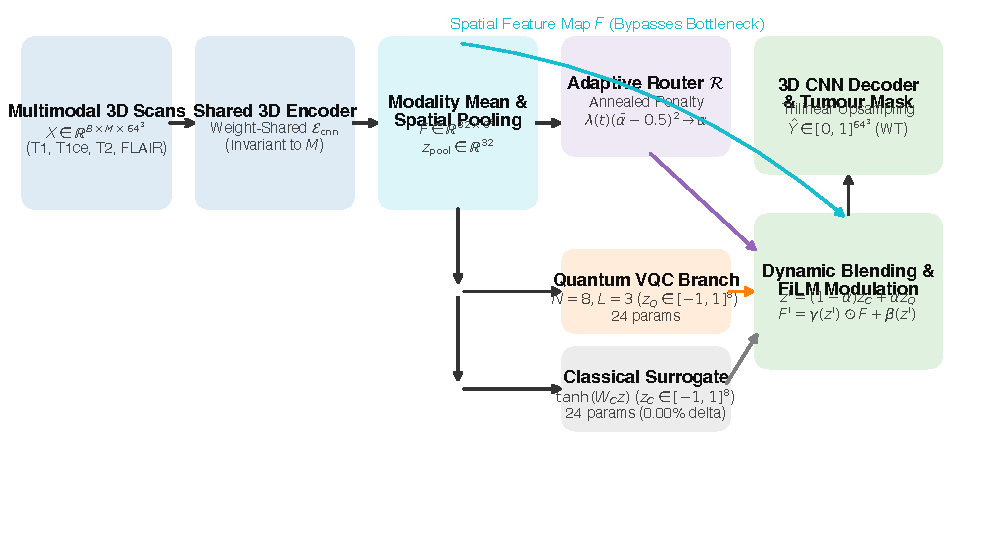
\includegraphics[width=\textwidth]{figures/fig1_architecture.pdf}
\caption{The Q-FUSION architecture. Volumetric multimodal inputs $X \in \mathbb{R}^{B \times M \times 64 \times 64 \times 64}$ are processed through a weight-shared 3D CNN encoder to extract modality-invariant spatial representations $F_m$, aggregated via mean pooling. A trainable gating router $\mathcal{R}$ regularized by an annealed exploration penalty computes a dynamic allocation scalar $\alpha(x) \in [0, 1]$ balancing the 24-parameter variational quantum circuit against a 24-parameter capacity-matched classical surrogate (0.0000\% parameter variance). The blended bottleneck representation $z'$ modulates the unflattened 3D spatial feature map via FiLM, preserving anatomical spatial geometry for 3D segmentation without high-capacity unflattening layers.}
\label{fig:architecture}
\end{figure}

The network consists of four coordinated components: (1) an $M$-channel parameter-invariant 3D CNN encoder, (2) parallel classical surrogate and variational quantum bottlenecks, (3) a dynamic classical-quantum gating router regularized by an annealed exploration penalty, and (4) a quantum-conditioned 3D spatial modulation decoder.

\subsection{Multimodal 3D Encoding and Channel Aggregation}
Let $X \in \mathbb{R}^{B \times M \times D \times H \times W}$ denote a batch of $B$ patient scans comprising $M$ co-registered volumetric modalities (where $M \in \{1, 2, 3, 4\}$). 
To enforce exact parameter invariance across arbitrary modality combinations, all $M$ channels are processed through a single, weight-shared 3D convolutional encoder $\mathcal{E}_{\text{cnn}}$:
\begin{equation}
    F_m = \mathcal{E}_{\text{cnn}}(X[:, m:m+1]), \quad m \in \{1, \dots, M\}
\end{equation}
where $F_m \in \mathbb{R}^{B \times C \times D' \times H' \times W'}$ represents the spatial feature map for modality $m$, with channel dimension $C=32$ and downsampled spatial resolution $8 \times 8 \times 8$.

The $M$ spatial representations are aggregated via channel-wise mean pooling:
\begin{equation}
    F = \frac{1}{M} \sum_{m=1}^M F_m \in \mathbb{R}^{B \times 32 \times 8 \times 8 \times 8}
\end{equation}
Global average spatial pooling is subsequently applied to extract a compact multimodal summary vector:
\begin{equation}
    z_{\text{pool}} = \text{AdaptiveAvgPool3D}(F) \in \mathbb{R}^{B \times 32}
\end{equation}
A linear compression projection maps $z_{\text{pool}}$ to the input vector $z_{\text{comp}} \in \mathbb{R}^{B \times 24}$ required by the parallel bottlenecks.

\subsection{Quantum Bottleneck: Sequential Data Re-uploading}
The quantum pathway comprises an $N$-qubit parameterized circuit with $L$ sequential data re-uploading layers \cite{perez2020data}. 
In our canonical configuration ($N=8$ qubits, $L=3$ layers), the input vector $z_{\text{comp}} \in \mathbb{R}^{24}$ is partitioned into three 8-dimensional chunks $z_{\text{comp}}^{(l)} \in \mathbb{R}^8$ for $l \in \{1, 2, 3\}$. 
At each layer $l$, the features are embedded via parameterized Pauli-Y rotations:
\begin{equation}
    U_{\text{enc}}(z_{\text{comp}}^{(l)}) = \bigotimes_{j=0}^{N-1} R_y\left(z_{\text{comp}, j}^{(l)}\right)
\end{equation}
Following data encoding, a parameterized entangling block transforms the register:
\begin{equation}
    U_{\text{ent}}(\theta^{(l)}) = \left( \prod_{j=0}^{N-1} \text{CNOT}_{(j, (j+1) \bmod N)} \right) \left( \bigotimes_{j=0}^{N-1} R_y\left(\theta_j^{(l)}\right) \right)
\end{equation}
where $\theta \in \mathbb{R}^{3 \times 8}$ denotes the trainable quantum weight tensor containing exactly 24 parameters. 
The circuit output is extracted via expectation values of the Pauli-Z observable across all $N$ qubits:
\begin{equation}
    z_{Q, j} = \langle 0^{\otimes N} | U^\dagger \sigma_z^{(j)} U | 0^{\otimes N} \rangle \in [-1, 1], \quad j \in \{0, \dots, N-1\}
\end{equation}
yielding the compact quantum bottleneck representation $z_Q \in \mathbb{R}^{B \times 8}$.

\subsection{Capacity-Matched Classical Surrogate Control}
To rigorously resolve the classical control objection (Section 16, Pitfall 3), we implement a capacity-matched classical surrogate bottleneck $\mathcal{S}_{\text{class}}$. 
The surrogate accepts the identical 24-dimensional input vector $z_{\text{comp}}$ and possesses an identical trainable parameter tensor $W_C \in \mathbb{R}^{3 \times 8}$ (exactly 24 parameters):
\begin{equation}
    z_C = \tanh\left( \sum_{l=0}^{2} W_C^{(l)} \odot z_{\text{comp}}^{(l)} \right) \in [-1, 1]^8
\end{equation}
The $\tanh$ non-linearity enforces exact range parity with the Pauli-Z expectation values ($[-1, 1]$), ensuring that the quantum and classical branches are mathematically capacity-matched with 0.0000\% parameter variance.

\subsection{Adaptive Gating Router and Annealed Anti-Collapse Loss}
The adaptive router $\mathcal{R}$ evaluates the pooled multimodal representation $z_{\text{pool}}$ to compute a continuous routing scalar $\alpha \in [0, 1]$:
\begin{equation}
    \alpha = \sigma\left( W_2 \cdot \text{ReLU}(W_1 z_{\text{pool}} + b_1) + b_2 \right) \in [0, 1]
\end{equation}
The blended latent bottleneck representation $z'$ is formed as a convex combination:
\begin{equation}
    z' = (1 - \alpha) z_C + \alpha z_Q \in \mathbb{R}^{B \times 8}
\end{equation}

\subsubsection{Resolution of Classical Collapse}
To prevent the gating router from prematurely collapsing to purely classical processing ($\alpha \to 0$) during early optimization, we formulate a time-dependent annealed routing objective:
\begin{equation}
    \mathcal{L}_{\text{total}}(t) = \mathcal{L}_{\text{task}}(y_{\text{pred}}, y_{\text{true}}) + \lambda(t) \cdot (\bar{\alpha} - 0.5)^2
\end{equation}
where $\mathcal{L}_{\text{task}}$ is a compound Binary Cross-Entropy and Soft Dice loss:
\begin{equation}
    \mathcal{L}_{\text{task}} = \mathcal{L}_{\text{BCE}}(y_{\text{pred}}, y_{\text{true}}) + \mathcal{L}_{\text{Dice}}(y_{\text{pred}}, y_{\text{true}})
\end{equation}
The regularization weight $\lambda(t)$ follows a piecewise linear annealing schedule:
\begin{equation}
    \lambda(t) = \max\left( \lambda_{\min}, \lambda_{\text{init}} - \frac{t}{T_{\text{decay}}} (\lambda_{\text{init}} - \lambda_{\min}) \right)
\end{equation}
with $\lambda_{\text{init}} = 1.0$, $\lambda_{\min} = 0.01$, and $T_{\text{decay}} = 10$ epochs. 
Early in training, $\lambda(t)$ penalizes deviations from an equal 50:50 allocation, forcing gradient descent to explore both branches. 
As training progresses, $\lambda(t)$ relaxes, allowing the router to settle on the empirical allocation ratio demanded by the data.

\subsection{Quantum-Conditioned Spatial Modulation (FiLM)}
To resolve the spatial reconstruction paradox without high-dimensional unflattening layers, the 8-dimensional bottleneck vector $z'$ modulates the unflattened 3D spatial feature map $F \in \mathbb{R}^{B \times 32 \times 8 \times 8 \times 8}$ using affine parameters:
\begin{equation}
    \gamma = \text{Linear}_{8 \to 32}(z'), \quad \beta = \text{Linear}_{8 \to 32}(z')
\end{equation}
\begin{equation}
    F' = \gamma \odot F + \beta
\end{equation}
The modulated feature map $F'$ is subsequently decoded by a 3D trilinear upsampling decoder to generate the final voxel-level probability volume $\hat{Y} \in [0, 1]^{B \times 1 \times 64 \times 64 \times 64}$.

\subsection{Simulated Open-System Quantum Noise}
To evaluate architectural resilience on NISQ hardware, we simulate physical gate depolarizing noise on density matrices $\rho$:
\begin{equation}
    \mathcal{E}_p(\rho) = (1 - p)\rho + \frac{p}{3} \sum_{k \in \{X, Y, Z\}} \sigma_k \rho \sigma_k
\end{equation}
The depolarizing channel $\mathcal{E}_p$ with parameter $p \in [0.000, 0.050]$ is applied across all $N$ qubits after each layer of parameterized entangling gates. 
Simulations execute on PennyLane's `default.mixed` backend using analytic density-matrix backpropagation.
